%------------------------------------------------------------
\section{Diffusore subsonico}
%------------------------------------------------------------
\label{app:presa_aria_subsonica}

Le condizioni di volo alla quota di progetto sono ricavate mediante il modello ISA e le relazioni riportate in Appendice~\ref{app:appendiceA.1}.

Nel modello viene considerata una presa d'aria non ideale. Il rendimento isentropico del diffusore viene imposto pari a

\begin{equation*}
\eta_d=0.975
\end{equation*}

Il corrispondente coefficiente di recupero della pressione totale è calcolato mediante la relazione 

\begin{equation*}
\pi_D=
\left(
\frac{
1+\eta_d\frac{\gamma_a-1}{2}M_0^2
}{
1+\frac{\gamma_a-1}{2}M_0^2
}
\right)^{\frac{\gamma_a}{\gamma_a-1}}
=0.989
\end{equation*}

Per l'ipotesi adiabatica la temperatura totale si conserva, mentre la perdita di pressione totale è introdotta mediante $\pi_D$:
\begin{equation*}
    T_{02}=T_{00}
\end{equation*}
\begin{equation*}
    P_{02}=\pi_D P_{00}
\end{equation*}

dove $T_{00}$ e $P_{00}$ sono le grandezze totali della corrente indisturbata, calcolate in Appendice~\ref{app:appendiceA.1}.


\subsection{Condizioni statiche all'uscita della presa d'aria}

All'uscita del diffusore è imposto un numero di Mach $M_2=0.5$. Le corrispondenti grandezze statiche sono determinate dalle relazioni isoentropiche:

\begin{equation*}
    T_2=
    \frac{T_{02}}
    {1+\frac{\gamma_a-1}{2}M_2^2}
\end{equation*}

\begin{equation*}
    P_2=
    \frac{P_{02}}
    {\left(1+\frac{\gamma_a-1}{2}M_2^2\right)^{\frac{\gamma_a}{\gamma_a-1}}}
\end{equation*}

La densità, la velocità del suono e la velocità del flusso risultano:

\begin{equation*}
    \rho_2=\frac{P_2}{R_aT_2}
\end{equation*}

\begin{equation*}
    a_2=\sqrt{\gamma_aR_aT_2}
\end{equation*}

\begin{equation*}
    V_2=M_2a_2
\end{equation*}


\subsection{Dimensionamento geometrico }

La sezione di ingresso della presa d'aria è determinata mediante l'equazione di continuità:

\begin{equation*}
A_0=
\frac{\dot{m}_{air}}
{\rho_0V_0}
\end{equation*}

La sezione all'uscita del diffusore, coincidente con la sezione di ingresso del compressore, risulta:

\begin{equation*}
A_2=
\frac{\dot{m}_{air}}
{\rho_2V_2}
\end{equation*}

Assumendo una sezione circolare, i diametri delle sezioni di ingresso e di uscita sono:

\begin{equation*}
D_1=
\sqrt{\frac{4A_0}{\pi}}
\end{equation*}

\begin{equation*}
D_2=
\sqrt{\frac{4A_2}{\pi}}
\end{equation*}

Dal rapporto tra le due sezioni si ricava:

\begin{equation*}
\frac{D_2}{D_1}
=
\sqrt{\frac{A_2}{A_0}}
\end{equation*}

Al fine di contenere la lunghezza del diffusore è stato adottato un rapporto geometrico costante pari a

\begin{equation*}
\frac{L}{D_1}=1.5.
\end{equation*}

L'angolo totale di divergenza viene quindi ricavato imponendo la geometria di un diffusore conico:

\begin{equation*}
\frac{D_2}{D_1}
=
1+
2\left(\frac{L}{D_1}\right)\tan\phi
\end{equation*}

da cui si ottiene l'angolo totale di divergenza:

\[
2\phi = 6.69^\circ.
\]

La configurazione individuata viene infine verificata mediante il diagramma riportato in Figura~\ref{fig:diffusoreSubsonico}. Il punto ottenuto ricade nella regione \emph{No appreciable stall}.

\begin{figure}[H]
    \centering
    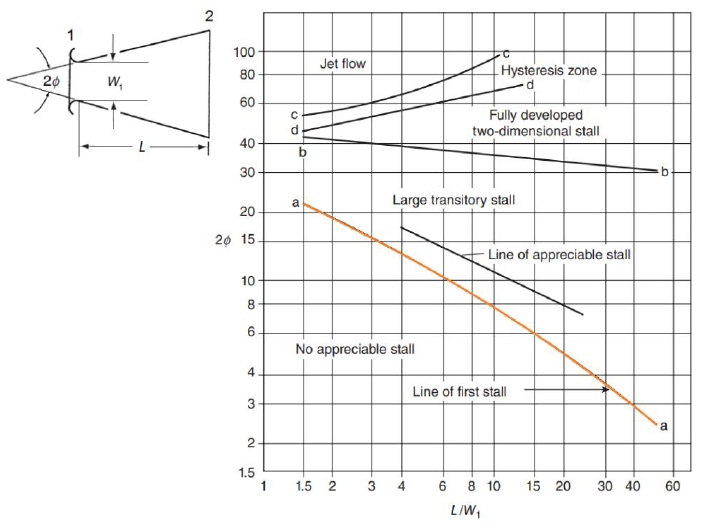
\includegraphics[width=0.82\linewidth]{Graphics/turbogetto/presaAria/Geometria_diffusore_subsonico.png}
    \caption{Diagramma utilizzato per la verifica della geometria del diffusore subsonico.}
    \label{fig:diffusoreSubsonico}
\end{figure}

La lunghezza del diffusore risulta infine:

\begin{equation*}
L=
\left(\frac{L}{D_1}\right)D_1.
\end{equation*}



%------------------------------------------------------------
\section{Compressore}
%------------------------------------------------------------
\label{app:compressore}
Il dimensionamento del compressore è stato effettuato a partire dalle
condizioni totali fornite dalla presa d'aria e dai parametri di progetto
$\pi_c$, $U_{tip}$ e $\eta_{p,c}$.

\subsection{Prestazioni termodinamiche}

Assumendo un rendimento politropico costante
$\eta_{p,c}=0.90$, il corrispondente rendimento isoentropico è

\begin{equation*}
\eta_c=
\frac{\pi_c^{\frac{\gamma_a-1}{\gamma_a}}-1}
{\pi_c^{\frac{\gamma_a-1}{\gamma_a\eta_{p,c}}}-1}.
\end{equation*}

Le condizioni totali all'uscita del compressore risultano

\begin{equation*}
P_{03}=\pi_c P_{02},
\end{equation*}

\begin{equation*}
T_{03s}=T_{02}\pi_c^{\frac{\gamma_a-1}{\gamma_a}},
\qquad
T_{03}=T_{02}+\frac{T_{03s}-T_{02}}{\eta_c}.
\end{equation*}

Il lavoro specifico e la potenza assorbita sono quindi

\begin{equation*}
l_c=c_{p,a}(T_{03}-T_{02}),
\qquad
\dot{L}_c=\dot{m}_{air}l_c.
\end{equation*}


\subsection{Dimensionamento Geometrico}

All'ingresso del compressore è imposto $M_2=0.5$. Le condizioni statiche
sono ricavate dalle corrispondenti grandezze totali:

\begin{equation*}
T_2=
\frac{T_{02}}
{1+\frac{\gamma_a-1}{2}M_2^2},
\qquad
P_2=
\frac{P_{02}}
{\left(1+\frac{\gamma_a-1}{2}M_2^2\right)^
{\frac{\gamma_a}{\gamma_a-1}}},
\end{equation*}

\begin{equation*}
\rho_2=\frac{P_2}{R_aT_2},
\qquad
a_2=\sqrt{\gamma_aR_aT_2},
\qquad
V_a=M_2a_2.
\end{equation*}

L'area anulare di ingresso è determinata dalla continuità:

\begin{equation*}
A_2=\frac{\dot{m}_{air}}{\rho_2V_a}.
\end{equation*}

Assumendo un rapporto mozzo-punta

\begin{equation*}
\lambda=\frac{r_{h,2}}{r_{t,2}}=0.5,
\end{equation*}

si ottengono

\begin{equation*}
r_{t,2}=
\sqrt{\frac{A_2}{\pi(1-\lambda^2)}},
\qquad
r_{h,2}=\lambda r_{t,2},
\end{equation*}

\begin{equation*}
r_{m,2}=\frac{r_{t,2}+r_{h,2}}{2},
\qquad
h_2=r_{t,2}-r_{h,2}.
\end{equation*}

Nota la velocità periferica di punta $U_{tip}$, ottenuta dal processo di
ottimizzazione,

\begin{equation*}
\omega=\frac{U_{tip}}{r_{t,2}},
\qquad
U=\omega r_{m,2}.
\end{equation*}

Assumendo velocità assiale e raggio di punta costanti lungo il
compressore, le condizioni statiche all'uscita sono

\begin{equation*}
T_3=T_{03}-\frac{V_a^2}{2c_{p,a}},
\qquad
a_3=\sqrt{\gamma_aR_aT_3},
\qquad
M_3=\frac{V_a}{a_3},
\end{equation*}

\begin{equation*}
P_3=
\frac{P_{03}}
{\left(1+\frac{\gamma_a-1}{2}M_3^2\right)^
{\frac{\gamma_a}{\gamma_a-1}}},
\qquad
\rho_3=\frac{P_3}{R_aT_3}.
\end{equation*}

La geometria della sezione di uscita è quindi determinata mediante

\begin{equation*}
A_3=\frac{\dot{m}_{air}}{\rho_3V_a},
\qquad
r_{t,3}=r_{t,2},
\end{equation*}

\begin{equation*}
r_{h,3}=
\sqrt{r_{t,3}^2-\frac{A_3}{\pi}},
\qquad
r_{m,3}=\frac{r_{t,3}+r_{h,3}}{2},
\qquad
h_3=r_{t,3}-r_{h,3}.
\end{equation*}


\subsection{Dimensionamento del primo stadio}

Il primo stadio è dimensionato al raggio medio assumendo velocità assiale
costante e ingresso assiale nel rotore:

\begin{equation*}
V_{\theta,1}=0,
\qquad
W_{\theta,1}=V_{\theta,1}-U,
\qquad
W_1=\sqrt{V_a^2+W_{\theta,1}^2}.
\end{equation*}

Per il dimensionamento preliminare viene imposto il limite di De Haller

\begin{equation*}
\frac{W_2}{W_1}=0.72,
\end{equation*}

da cui

\begin{equation*}
W_2=0.72W_1,
\qquad
W_{\theta,2}=-\sqrt{W_2^2-V_a^2},
\qquad
V_{\theta,2}=W_{\theta,2}+U.
\end{equation*}

Applicando l'equazione di Eulero, il lavoro specifico teorico dello
stadio risulta

\begin{equation*}
l_{st,teo}=U(V_{\theta,2}-V_{\theta,1}),
\end{equation*}

da cui viene stimato il numero di stadi:

\begin{equation*}
N_{stadi}
=
\left\lceil
\frac{l_c}{l_{st,teo}}
\right\rceil.
\end{equation*}

Poiché $N_{stadi}$ deve assumere un valore intero, il lavoro specifico
viene successivamente ridistribuito uniformemente tra gli stadi:

\begin{equation*}
l_{st}=\frac{l_c}{N_{stadi}},
\end{equation*}

e il triangolo di velocità viene ricalcolato mediante

\begin{equation*}
V_{\theta,2}
=
V_{\theta,1}+\frac{l_{st}}{U}.
\end{equation*}

Le velocità risultanti sono quindi

\begin{align*}
V_1 &= \sqrt{V_a^2+V_{\theta,1}^2}, &
V_2 &= \sqrt{V_a^2+V_{\theta,2}^2},\\
W_{\theta,1} &= V_{\theta,1}-U, &
W_{\theta,2} &= V_{\theta,2}-U,\\
W_1 &= \sqrt{V_a^2+W_{\theta,1}^2}, &
W_2 &= \sqrt{V_a^2+W_{\theta,2}^2}.
\end{align*}

Il fattore di De Haller finale viene pertanto verificato sul triangolo
ricalcolato e può risultare superiore al valore limite inizialmente
imposto.


\subsection{Verifiche aerodinamiche}

Sul triangolo di velocità ricalcolato vengono valutati

\begin{equation*}
DeHaller=\frac{W_2}{W_1},
\qquad
C_p=1-\left(\frac{W_2}{W_1}\right)^2,
\end{equation*}

e gli angoli relativi del rotore

\begin{equation*}
\beta_1=\arctan\left(\frac{W_{\theta,1}}{V_a}\right),
\qquad
\beta_2=\arctan\left(\frac{W_{\theta,2}}{V_a}\right).
\end{equation*}

I massimi numeri di Mach assoluto e relativo sono

\begin{equation*}
M_{abs}=
\max\left(\frac{V_1}{a_2},\frac{V_2}{a_2}\right),
\qquad
M_{rel}=
\max\left(\frac{W_1}{a_2},\frac{W_2}{a_2}\right).
\end{equation*}

Assumendo $\sigma_r=1.0$ e $\sigma_s=1.25$, i coefficienti di
diffusione di rotore e statore sono

\begin{equation*}
D_r=
1-\frac{W_2}{W_1}
+
\frac{|V_{\theta,2}-V_{\theta,1}|}
{2\sigma_r W_1},
\end{equation*}

\begin{equation*}
D_s=
1-\frac{V_a}{V_2}
+
\frac{|V_{\theta,2}-V_{\theta,1}|}
{2\sigma_s V_2}.
\end{equation*}

Il grado di reazione al raggio medio è

\begin{equation*}
R=
1-\frac{V_{\theta,1}+V_{\theta,2}}{2U}.
\end{equation*}


\subsection{Numero di pale rotoriche}

La corda al raggio medio viene determinata imponendo

\begin{equation*}
Re_c=\frac{W_1c_m}{\nu}\geq 3\times10^5.
\end{equation*}

Assumendo il valore limite,

\begin{equation*}
c_m=\frac{3\times10^5\,\nu}{W_1}.
\end{equation*}

Dalla solidity rotorica $\sigma_r=c_m/s_r=1$ segue

\begin{equation*}
s_r=\frac{c_m}{\sigma_r},
\end{equation*}

e il numero di pale viene determinato come

\begin{equation*}
N_{pale,r}
=
\left\lceil
\frac{2\pi r_{m,2}}{s_r}
\right\rceil.
\end{equation*}


\section{Diffusore}
\label{app:diffusore}

Si riporta di seguito la catena di calcolo completa alla base dei risultati del diffusore di raccordo compressore-camera, presentati nella Sezione~\ref{sec:camera}.

Le condizioni di ingresso ($T_{03}$, $P_{03}$, $M_3$) coincidono con le grandezze totali e il numero di Mach in uscita dal compressore. La temperatura totale si conserva lungo il condotto (trasformazione adiabatica), mentre la pressione totale è ridotta dal rendimento pneumatico assegnato:
\begin{equation*}
    T_{03.5} = T_{03}, \qquad P_{03.5} = \pi_d\,P_{03}.
\end{equation*}

Le grandezze statiche in ingresso, necessarie per il calcolo dell'area di passaggio, si ottengono dalle relazioni isoentropiche applicate al Mach $M_3$:
\begin{equation*}
    T_3 = \frac{T_{03}}{1+\dfrac{\gamma-1}{2}M_3^2}, \qquad
    P_3 = \frac{P_{03}}{\left(1+\dfrac{\gamma-1}{2}M_3^2\right)^{\gamma/(\gamma-1)}}, \qquad
    \rho_3 = \frac{P_3}{R\,T_3},
\end{equation*}
da cui la velocità $v_3 = M_3\sqrt{\gamma R T_3}$ e, per continuità, la sezione di ingresso:
\begin{equation*}
    A_3 = \frac{\dot{m}_{aria}}{\rho_3\,v_3}.
\end{equation*}

Le medesime relazioni, valutate sul Mach di uscita imposto $M_{3.5}$ e sulle grandezze totali $T_{03.5}$, $P_{03.5}$, forniscono le condizioni statiche e la sezione di uscita:
\begin{equation*}
    T_{3.5} = \frac{T_{03.5}}{1+\dfrac{\gamma-1}{2}M_{3.5}^2}, \qquad
    P_{3.5} = \frac{P_{03.5}}{\left(1+\dfrac{\gamma-1}{2}M_{3.5}^2\right)^{\gamma/(\gamma-1)}}, \qquad
    \rho_{3.5} = \frac{P_{3.5}}{R\,T_{3.5}},
\end{equation*}
\begin{equation*}
    v_{3.5} = M_{3.5}\sqrt{\gamma R T_{3.5}}, \qquad A_{3.5} = \frac{\dot{m}_{aria}}{\rho_{3.5}\,v_{3.5}}.
\end{equation*}

Assumendo una geometria anulare con raggio medio $r_{medio}$ coincidente con quello dell'ultimo stadio del compressore, le altezze del canale in ingresso e in uscita si ricavano da
\begin{equation*}
    h_3 = \frac{A_3}{2\pi\,r_{medio}}, \qquad h_{3.5} = \frac{A_{3.5}}{2\pi\,r_{medio}}.
\end{equation*}

La lunghezza assiale del diffusore è infine determinata imponendo il semi-angolo di apertura $\theta$, in modo da limitare il rischio di distacco dello strato limite lungo le pareti divergenti:
\begin{equation*}
    L_D = \frac{h_{3.5}-h_3}{2\tan\theta}.
\end{equation*}

%------------------------------------------------------------
\section{Camera di Combustione}
%------------------------------------------------------------
\label{app:camera_combustione}


Si riporta di seguito la catena di calcolo completa alla base dei risultati presentati nella Sezione~\ref{sec:camera}, relativa al modello a doppia zona del combustore anulare nel punto di progetto turbogetto.

\subsection{Grandezze statiche in ingresso}

Le condizioni disponibili a valle del diffusore ($P_{03}'$, $T_{03}'$, $M_{03}'$) sono espresse in termini di grandezze totali. Il calcolo della densità del flusso in ingresso alla camera richiede le corrispondenti grandezze statiche, ottenute mediante le relazioni isoentropiche:
\begin{equation*}
    T_3 = \frac{T_{03}'}{1 + \dfrac{\gamma_a - 1}{2} M_{03}'^2}, \qquad
    P_3 = \frac{P_{03}'}{\left(1 + \dfrac{\gamma_a - 1}{2} M_{03}'^2\right)^{\gamma_a/(\gamma_a - 1)}}, \qquad
    \rho_3 = \frac{P_3}{R_a T_3}.
\end{equation*}

\subsection{Rapporti combustibile/aria e rapporto di equivalenza}

Applicando il bilancio entalpico separatamente nella zona primaria (a temperatura $T_{comb}$) e sull'intero sistema (a temperatura $T_{04}$) si ottengono rispettivamente il rapporto combustibile/aria locale e quello globale:
\begin{equation*}
    f_{liner} = \frac{c_{p,g}\,T_{comb} - c_{p,a}\,T_{03}'}{LHV\,\eta_b - c_{p,g}\,T_{comb} + c_{p,f}\,T_{fuel}}, \qquad
    f_{global} = \frac{c_{p,g}\,T_{04} - c_{p,a}\,T_{03}'}{LHV\,\eta_b - c_{p,g}\,T_{04} + c_{p,f}\,T_{fuel}},
\end{equation*}
con $T_{fuel} = 273.15$ K temperatura di ingresso del combustibile. Il rapporto di equivalenza della zona primaria segue come
\begin{equation*}
    \phi = \frac{f_{liner}}{f_{st}}, \qquad f_{st} = 0.068.
\end{equation*}

\subsection{Suddivisione delle portate d'aria}

La frazione di portata che alimenta la zona primaria si ricava imponendo la conservazione dell'entalpia nella miscelazione adiabatica tra i gas a $T_{comb}$ e l'aria fredda by-passata a $T_{03}'$:
\begin{equation*}
    \dot{m}_{air,calda}\left(c_{p,g}T_{comb} - c_{p,a}T_{03}'\right) = \dot{m}_{air}\left(c_{p,g}T_{04} - c_{p,a}T_{03}'\right)
    \ \Longrightarrow \
    \dot{m}_{air,calda} = \dot{m}_{air}\,\frac{c_{p,g}T_{04} - c_{p,a}T_{03}'}{c_{p,g}T_{comb} - c_{p,a}T_{03}'},
\end{equation*}
da cui $\dot{m}_{air,fredda} = \dot{m}_{air} - \dot{m}_{air,calda}$. Portata di combustibile e calore rilasciato risultano
\begin{equation*}
    \dot{m}_{comb} = f_{global}\,\dot{m}_{air}, \qquad \dot{Q} = \dot{m}_{comb}\,LHV\,\eta_b.
\end{equation*}

\subsection{Dimensionamento trasversale}

Dalla correlazione $\Delta P/q_{ref} = \text{cost}$ si ricava la sezione di riferimento:
\begin{equation*}
    A_{ref} = \sqrt{\frac{R_g}{2}\left(\frac{\dot{m}_{air}\sqrt{T_{03}'}}{P_{03}'}\right)^2 \frac{k_{din}}{\Delta P/P_{03}'}},
\end{equation*}
con $k_{din}$ coefficiente di perdita dinamica. Dal raggio medio anulare ereditato dal compressore, $r_{medio} = r_{M3}$, si ottiene l'altezza del canale $h_{ref} = A_{ref}/(2\pi\,r_{medio})$, mentre le grandezze di verifica nella sezione di riferimento sono
\begin{equation*}
    U_{ref} = \frac{\dot{m}_{air}}{\rho_3\,A_{ref}}, \qquad q_{ref} = \frac{1}{2}\rho_3 U_{ref}^2, \qquad M_{ref} = \frac{U_{ref}}{\sqrt{\gamma_g R_g T_{03}'}}.
\end{equation*}
Per il calcolo del tempo di residenza sono necessarie le grandezze locali nel liner, ottenute scalando l'area di riferimento sulla sola frazione di portata calda:
\begin{equation*}
    A_{liner} = A_{ref}\,\frac{\dot{m}_{air,calda}}{\dot{m}_{air}}, \qquad \rho_{liner} = \frac{P_3}{R_g\,T_{comb}}, \qquad U_{liner} = \frac{\dot{m}_{air,calda} + \dot{m}_{comb}}{A_{liner}\,\rho_{liner}}.
\end{equation*}

\subsection{Dimensionamento volumetrico, longitudinale e verifica del tempo di residenza}

Dal vincolo sull'intensità di combustione $I = \dot{Q}/(V\,P_{03}')$ si ricava il volume della camera e, nota $A_{ref}$, la lunghezza assiale:
\begin{equation*}
    V = \frac{\dot{Q}}{I\,P_{03}'}, \qquad L_c = \frac{V}{A_{ref}}.
\end{equation*}
Il tempo di residenza nella zona primaria, confrontato con il vincolo $t_{res} > 8$ ms imposto in ottimizzazione, è dato da
\begin{equation*}
    t_{res} = \frac{L_c}{U_{ref}}.
\end{equation*}

\subsection{Condizioni di uscita}

Pressione e temperatura totali in uscita dalla camera risultano
\begin{equation*}
    P_{04} = \left(1 - \frac{\Delta P}{P_{03}'}\right)P_{03}', \qquad T_{04} = \text{TIT imposta in ottimizzazione (Sezione 1.2)}.
\end{equation*}

Di seguito viene schematizzata la ripartizione del flusso d'aria e le successive fasi di trasformazione termodinamica all'interno della camera di combustione:
\begin{figure}[H]
    \centering
    \resizebox{\textwidth}{!}{%
    \begin{tikzpicture}[
        node distance = 10mm and 14mm,
        box/.style = {rectangle, draw, rounded corners=2pt, minimum width=30mm, minimum height=11mm,
                       align=center, font=\small, fill=gray!8},
        arr/.style = {-{Latex[length=2mm]}, thick},
        lbl/.style = {font=\scriptsize, align=center, fill=white, inner sep=1pt}
    ]

        \node[box] (diff) {Diffusore\\(uscita)\\[1pt]\footnotesize $T_{03}'$, $P_{03}'$};

        \node[box, above right=14mm and 24mm of diff, fill=orange!12] (liner) {Zona primaria\\(liner)\\[1pt]\footnotesize $T_{comb}$};

        \node[box, below right=14mm and 24mm of diff, fill=teal!10] (dil) {Aria di\\diluizione\\[1pt]\footnotesize $T_{03}'$};

        \node[box, right=24mm of diff, fill=violet!10] (mix) at ($(liner)!0.5!(dil)+(24mm,0)$) {Miscelazione\\adiabatica};

        \node[box, right=14mm of mix, fill=gray!15] (out) {Uscita\\camera\\[1pt]\footnotesize $T_{04}$, $P_{04}$};

        \node[above=6mm of liner, font=\scriptsize] (fuel) {JP-7};

      
        \draw[arr] (diff.east) -- ++(6mm,0) |- (liner.west) node[lbl, pos=0.3, above] {$\dot{m}_{air,calda}$};
        \draw[arr] (diff.east) -- ++(6mm,0) |- (dil.west) node[lbl, pos=0.3, below] {$\dot{m}_{air,fredda}$};
        \draw[arr] (fuel) -- (liner.north) node[lbl, midway, right] {$\dot{m}_{comb}$};

    
        \draw[arr] (liner.south) -- ++(0,-5mm) -| (mix.north);
   
        \draw[arr] (dil.north) -- ++(0,5mm) -| (mix.south);

        \draw[arr] (mix.east) -- (out.west) node[lbl, midway, above] {$\dot{m}_{gas}$};

        % Portata totale in ingresso
        \node[lbl, above=1mm of diff, fill=none] {$\dot{m}_{air}$};

    \end{tikzpicture}%
    }
    \caption{Schema funzionale della camera di combustione e ripartizione delle portate massiche.}
    \label{fig:schema_camera}
\end{figure}



%------------------------------------------------------------
\section{Turbina}
%------------------------------------------------------------
\label{appB:turbina}

Il lavoro prodotto dalla turbina è calcolato applicando un rendimento al lavoro del compressore. Tale rendimento serve a tenere conto degli attriti meccanici e di tutti i sistemi che richiedono potenza generata dalla turbina (elettrico, idraulico...). Pertanto viene applicato il rendimento meccanico $\eta_m = 0.95$:
\begin{equation*}
   \dot{L}_{\text{turbina}} = \frac{\dot{L}_{\text{compressore}}}{\eta_m}
\end{equation*}

Si definisce la frazione di aria spillata dal compressore come:
\begin{equation*}
    x_{\text{spillaggio}}(T_{\text{04}}) = \frac{\dot{m}_{\text{spillata}}}{\dot{m}_{\text{totale}}} 
\end{equation*}

Tale grandezza è funzione della temperatura di combustione del turbogetto e si ricava tramite Appendice~\ref{ap:appendixA}. Notare che la $\dot{m}_\text{totale}$ corrisponde alla portata totale in uscita dal motore, mentre la percentuale ricavata in Appendice ~\ref{ap:appendixA} corrisponde alla percentuale di aria spillata dal compressore. Pertanto:
\begin{equation*}
    x_\text{spillaggio} = \frac{x_\text{spillata(SOT)}\dot{m}_\text{aria}}{\dot{m}_\text{totale}}
\end{equation*}



La portata in uscita dalla camera di combustione si esprime come:
\begin{equation*}
    \dot{m}_{\text{camera}} = (1 - x_{\text{spillaggio}}) \dot{m}_{\text{totale}} 
\end{equation*}

\textbf{Grandezze totali all'uscita della turbina}\\
Applicando la conservazione dell'energia per un sistema aperto in condizioni
stazionarie, l'equazione di bilancio si riduce a:
\begin{align*}
    \frac{dE}{dt} &= \sum_{k}\dot{m}_k h_{0,k} + \dot{Q}^{\leftarrow} - \dot{L}^{\rightarrow} = 0 \\
    &= \dot{m}_{\text{camera}} c_{p,\text{g}} T_{04} + \dot{m}_{\text{spillata}} c_{p,\text{a}} T_{03} - \dot{m}_{\text{totale}} c_{p,\text{g}} T_{05} +\dot{Q}_{\text{turbina}}- \dot{L}_{\text{turbina}}  = 0
\end{align*}
Facendo l'ipotesi di turbina adiabatica e riarrangiando l'equazione di bilancio per esplicitare la temperatura di fine espansione $T_{05}$, si ottiene:
\begin{equation*}
    T_{05} = T_{04} (1 - x_{\text{spillaggio}}) + x_{\text{spillaggio}} \frac{c_{p,\text{a}}}{c_{p,\text{g}}} T_{03} - \frac{\dot{L}_{\text{compressore}}}{\dot{m}_{\text{totale}} c_{p,\text{g}} \eta_m}
\end{equation*}

Infine, applicando la relazione di espansione isoentropica mediante il rendimento politropico pari a $\eta_{\text{p,t}}$ = 0.9, si ricava il rapporto di pressione della turbina $\beta_{\text{turbina}}$:
\begin{equation*}
\beta_{\text{turbina}} = \left( \frac{T_{05}}{T_{04}} \right)^{\frac{\gamma_g}{(\gamma_g-1)\eta_{\text{p,t}}}}
\label{eqAPP:betaTurbinaCalc}
\end{equation*}
La pressione totale all'uscita della turbina si calcola come:
\begin{equation*}
P_{05} = \beta_{\text{turbina}} P_{04}
\end{equation*}

Il rendimento isoentropico della turbina è definito come:
\begin{equation*}
    \eta_t = \frac{\dot{L}_{\text{reale}}}{\dot{L}_{\text{ideale}}} = \frac{1 - \beta^{\frac{\gamma-1}{\gamma} \eta_{\text{p,t}}}}{1 - \beta^{\frac{\gamma-1}{\gamma}}}
\end{equation*}

\subsection{Stadio della turbina}
L'analisi è focalizzata sul singolo stadio (primo stadio) i cui parametri operativi sono successivamente estesi per determinare il numero di stadi complessivi della turbina.
Nello sviluppo del modello si assumono le seguenti ipotesi semplificative:
\begin{itemize}
\item Si trascura ogni perdita di pressione nello statore e nel rotore. Di conseguenza, la componente assiale della velocità è considerata costante ($v_{z} = \text{cost}$).
\item Il raggio medio della turbina coincide con il raggio medio dell'ultimo stadio del compressore.
\item Si considera un turbogetto a singolo albero, pertanto la velocità angolare $\omega$ della turbina coincide con quella del compressore.
\end{itemize}

Per permettere di calcolare le grandezze nello stadio di una turbina raffreddata si applica una semplificazione: una miscelazione adiabatica a pressione totale costante dopo lo statore del primo stadio con tutta l'aria di raffreddamento. Tale temperatura si calcola come:
\begin{equation}
T_{0M} = \frac{(1 - x_{\text{spillaggio}}) c_{p,g} T_{04} + x_{\text{spillaggio}} c_{p,a} T_{\text{spillaggio}}}{(1 - x_{\text{spillaggio}}) c_{p,g} + x_{\text{spillaggio}} c_{p,a}}
\label{appB:turbina:eq:miscelazione}
\end{equation}
La pressione totale $P_{0M}$ rimane invariata pari a $P_{04}.$ Inoltre si è ipotizzato che per tale miscelazione le velocità non vengono influenzate. 

Per chiarezza, nella turbina le proprietà nello statore/rotore hanno la seguente nomenclatura:
\begin{itemize}
    \item $[var]_1 \,\,\,=$ proprietà all'ingresso dello statore
    \item $[var]_\text{1.5} =$ proprietà all'uscita dello statore equivalenti all'ingresso del rotore
    \item $[var]_\text{2}\,\,\,=$ proprietà all'uscita del rotore
\end{itemize}

Notare che, nella divisione tra statore e rotore (1.5) vengono usati i pedici 's' statore e 'r' rotore per differenziare l'uscita dello statore con l'entrata del rotore. 


\subsection{Dimensionamento dello statore}
Nelle turbine, lo statore è utilizzato per orientare il flusso per il corretto ingresso nel rotore e in certe configurazioni il fluido viene espanso convertendo entalpia in energia cinetica. Il numero di Mach in uscita dallo statore è imposto pari a Mach = 1. Invece, le condizioni all'ingresso dello statore sono imposte dalla camera di combustione, in particolare il numero di Mach è compreso tra $0.4$ e $0.5$.

Le proprietà statiche d'ingresso si calcolano dalle grandezze totali mediante le relazioni isoentropiche:

\begin{equation*}
T_1 = T_{04} \left( 1 + \frac{\gamma_g - 1}{2} M_1^2 \right)^{-1}
\end{equation*}
\begin{equation*}
P_1= P_{04} \left( 1 + \frac{\gamma_g - 1}{2} M_1^2 \right)^{-\frac{\gamma_g}{\gamma_g - 1}} 
\end{equation*}
\begin{equation*}
    \rho_1 = \frac{P_1}{R_g T_1} 
\end{equation*}
\begin{equation*}
    v_1 = M_1 \sqrt{\gamma_g R_g T_1} 
\end{equation*}
\begin{equation*}
    A_1 = \frac{\dot{m}_\text{totale}(1-x_\text{spillaggio})}{\rho_1 v_1}
\end{equation*}


La sezione di uscita si calcola imponendo condizioni soniche all'uscita.

\begin{equation*}
T_{1.5,s} = T_{04} \left( 1 + \frac{\gamma_g - 1}{2} \right)^{-1}
\end{equation*}
\begin{equation*}
    P_{1.5,s} = P_{04} \left( 1 + \frac{\gamma_g - 1}{2} \right)^{-\frac{\gamma_g}{\gamma_g - 1}} 
\end{equation*}
\begin{equation*}
    \rho_{1.5,s} = \frac{P_{1.5,s}}{(R_g T_{1.5,s})}   
\end{equation*}
\begin{equation*}
    v_{1.5} = \sqrt{\gamma_g R_g T_{1.5,s}}
\end{equation*}
\begin{equation*}
    A_{t} = \frac{\dot{m}_\text{totale}(1-x_\text{spillaggio})}{\rho_{1.5,s} v_{1.5}}
\end{equation*}


Data la conservazione della velocità assiale, si ricavano la velocità trasversale e il relativo angolo con l'asse assiale. Pertanto:
\begin{align*}
    &v_{\theta,1.5} = \sqrt{v_{1.5}^2-v_{z,1.5}^2} =  \sqrt{v_{1.5}^2-v_{z}^2} \\
    &\alpha_{1.5}  \,\,=\arctan\left(\frac{v_{\theta,1.5}}{v_{z,1.5}}\right)
\end{align*}

\subsection{Dimensionamento del rotore}
Per la sezione di ingresso del rotore si prende in considerazione la velocità $v_\text{z} = v_\text{z,1.5}$ dato che il rotore è in rotazione. Dato che si applica una miscelazione adiabatica per simulare il raffreddamento dopo lo statore (equazione \ref{appB:turbina:eq:miscelazione}), vengono calcolate le temperature e pressioni totali e statiche per calcolare l'area di ingresso dello statore. 
\begin{equation*}
T_{1.5,r} = T_{0M} - \frac{v_{1.5}^2}{2cp_g}
\end{equation*}
\begin{equation*}
    M_{1.5,r} = \frac{v_{1.5}}{\sqrt{\gamma_gR_gT_{1.5,r}}}
\end{equation*}
\begin{equation*}
P_{1.5,r}= P_{0M} \left( 1 + \frac{\gamma_g - 1}{2} M_{1.5,r}^2 \right)^{-\frac{\gamma_g}{\gamma_g - 1}} 
\end{equation*}
\begin{equation*}
    \rho_{1.5,r} = \frac{P_{1.5,r}}{R_g T_{1.5,r}} 
\end{equation*}
\begin{equation*}
    A_{{1.5,r}} = \frac{\dot{m}_\text{totale}}{\rho_{{1.5,r}} v_{z,1.5}}
\end{equation*}

Si ricava il raggio di punta e del mozzo:
\begin{align*}
    h_{1.5} &= \frac{A_{1.5}}{2 \pi r_m} \\[6pt]
    r_{t,1.5} &= r_m + \frac{h_{1.5}}{2} \\[6pt]
r_{h,1.5} &= r_m - \frac{h_{1.5}}{2}
\end{align*}

Le velocità relative del rotore si calcolano mediante la seguente formula:
\begin{equation}
\vec{v} = \vec{w} + \vec{U}
\label{appB:eq:turbina:velocità}
\end{equation}
In particolare si calcola $w_{1.5}$ come:
\begin{equation*}
    \begin{cases}  w_{\theta,1.5} = v_{\theta,1.5} - U \\  w_{z,1.5} = v_{z,1.5} \end{cases}
\end{equation*}
La velocità U è equivalente alla velocità delle palette al raggio medio dell'ultimo stadio del compressore. Tra il compressore 
Come già discusso nella Sezione \ref{sec:turbina}, la velocità relativa in uscita dal rotore è imposta pari a Mach 0.9. Risolvendo per la velocità relativa $w_2$ utilizzando la conservazione dell'energia nel sistema di riferimento relativo:
\begin{equation*}
    a_{1.5,r} = \sqrt{\gamma_gR_gT_{1.5,r}}
\end{equation*}
\begin{equation*}
    M_{w,1.5} = \frac{\omega_{1.5}}{a_{1.5,r}}
\end{equation*}
\begin{equation*}
    w_{2} = \sqrt{\frac{a_{\text{1.5,r}}^2 + \frac{\gamma_g - 1}{2} w_{\text{1.5}}^2}{\frac{\gamma_g - 1}{2} + \frac{1}{M_{w,2}^2}}}
\end{equation*} 

Le componenti $w_\theta$ e la velocità $v_2$ si calcolano mediante Pitagora e l'equazione \eqref{appB:eq:turbina:velocità}:
\begin{equation*}
    \omega_{\theta,2} = -\sqrt{\omega _2^2-\omega_{z,2}^2} = -\sqrt{\omega _2^2-v_{z}^2}
\end{equation*}
\begin{equation*}
    \begin{cases}  v_{\theta,2} = \omega_{\theta,2} + U \\  v_{z,2} = \omega_{z,2} \end{cases}
\end{equation*}
    
Conoscendo le velocità si calcolano le proprietà termodinamiche all'uscita del rotore utilizzando l'equivalenza tra il lavoro calcolato in termini delle turbomacchine e in senso termodinamico. Si ricava che:
\begin{equation*}
T_{02} = T_{0M} - \frac{U (v_{\theta,1.5} - v_{\theta,2})}{c_{p,g}}
\end{equation*}
La pressione totale si calcola tramite una trasformazione isoentropica e viene poi utilizzata per calcolare le grandezze statiche da cui, mediante l'equazione di continuità, si calcola la grandezza dell'area all'uscita. La velocità utilizzata nell'equazione di continuità è di nuovo la sola velocità assiale.

\begin{equation*}
T_2 = T_{02} - \frac{v_2^2}{2cp_g}
\end{equation*}
\begin{equation*}
    M_2 = \frac{v_2}{\sqrt{\gamma_gR_gT_2}}
\end{equation*}
\begin{equation*}
    P_{02} = P_{0M} \left(\frac{T_{02}}{T_{0M}}\right)^{\frac{\gamma_g}{\gamma_g-1}}
\end{equation*}
\begin{equation*}
P_2= P_{02} \left( 1 + \frac{\gamma_g - 1}{2} M_2^2 \right)^{-\frac{\gamma_g}{\gamma_g - 1}} 
\end{equation*}
\begin{equation*}
    \rho_2 = \frac{P_2}{R_g T_2} 
\end{equation*}
\begin{equation*}
    A_2 = \frac{\dot{m}_\text{totale}}{\rho_2 v_{z,2}}
\end{equation*}

Si ricava il raggio di punta e del mozzo:
\begin{align*}
    h_{2} &= \frac{A_{2}}{2 \pi r_m} \\[6pt]
    r_{t,2} &= r_m + \frac{h_{2}}{2} \\[6pt]
r_{h,2} &= r_m - \frac{h_{2}}{2}
\end{align*}

Il lavoro del singolo stadio si calcola utilizzando le velocità all'ingresso e all'uscita dello statore:
\begin{equation*}
    L_{\text{stadio}} = U \left( v_{\theta,1.5} - v_{\theta,2} \right) \dot{m}_{\text{totale}}
\end{equation*}
Da tale relazione si ricava il numero di stadi della turbina, il primo stadio è uno stadio rappresentativo degli stadi, utilizzato per stimare il numero di stadi:
\begin{equation*}
    n_{\text{stadi}} = \left\lceil \frac{L_{\text{turbina}}}{L_{\text{stadio}}} \right\rceil 
\end{equation*}
Il grado di reazione della turbina invece si calcola tramite la seguente equazione:
\begin{equation*}
R = 1 - \frac{v_{\theta,1.5} + v_{\theta,2}}{2U}
\end{equation*}


\subsection{Sezioni Turbina}
La sezione di ingresso e di uscita della turbina si calcola utilizzando l'equazione di continuità. In particolare, conoscendo la velocità assiale $v_z$, le proprietà statiche si calcolano come:
\begin{equation*}
    T_4 = T_{04} -\frac{v_z^2}{2c_{p,g}}
\end{equation*}
\begin{equation*}
    M_4 = \frac{v_z}{\sqrt{\gamma_gR_gT_4}}
\end{equation*}
\begin{equation*}
    P_4 =  P_{04} \left( 1 + \frac{\gamma_g - 1}{2} M_4^2 \right)^{-\frac{\gamma_g}{\gamma_g - 1}} 
\end{equation*}
\begin{equation*}
    \rho_4 = \frac{P_4}{R_g T_4} 
\end{equation*}
\begin{equation*}
    A_4 = \frac{\dot{m}_\text{totale}(1-x_\text{spillaggio})}{\rho_4 v_z}
\end{equation*}

Per l'uscita:
\begin{equation*}
    T_5 = T_{05} -\frac{v_z^2}{2c_{p,g}}
\end{equation*}
\begin{equation*}
    M_5 = \frac{v_z}{\sqrt{\gamma_gR_gT_5}}
\end{equation*}
\begin{equation*}
    P_5 =  P_{05} \left( 1 + \frac{\gamma_g - 1}{2} M_5^2 \right)^{-\frac{\gamma_g}{\gamma_g - 1}} 
\end{equation*}
\begin{equation*}
    \rho_5 = \frac{P_5}{R_g T_5} 
\end{equation*}
\begin{equation*}
    A_5 = \frac{\dot{m}_\text{totale}}{\rho_5 v_z}
\end{equation*}

Si ricava il raggio di punta e del mozzo:
\begin{align*}
    h_5 &= \frac{A_5}{2 \pi r_m} \\[6pt]
    r_{t,5} &= r_m + \frac{h_5}{2} \\[6pt]
r_{h,5} &= r_m - \frac{h_5}{2}
\end{align*}

\subsection{Controllo dell'angolo ottimo}
L'angolo ottimo di uscita del flusso dallo statore dipende dal numero di Mach in ingresso. In particolare, tramite la Figura \ref{appB:turbina:fig:alphaottimo}, è possibile ricavare l'angolo $\alpha$ ottimo per un numero di Mach in ingresso pari a 0,5 e in uscita pari a 1.

\begin{figure}[H]
    \centering
    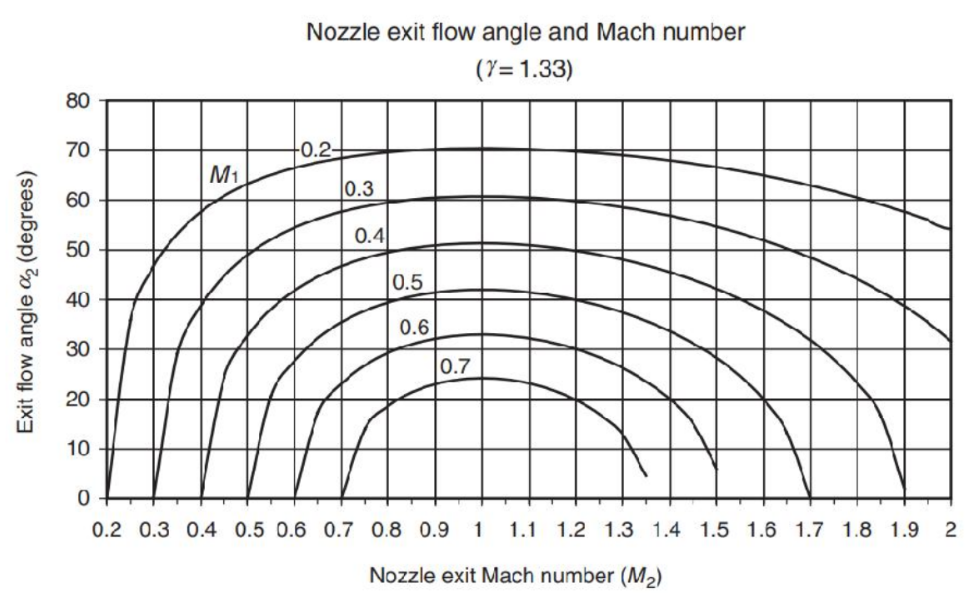
\includegraphics[width=0.7\linewidth]{Graphics/turbogetto/turbina/nozzleExit.png}
    \caption{Rappresentazione dell'angolo $\alpha$ ottimo in funzione del numero di Mach in ingresso e in uscita della turbina.}
    \label{appB:turbina:fig:alphaottimo}
\end{figure}

Per un Mach in ingresso di 0.5 l'angolo massimo risulta pari a 44°. Tale valore differisce da quello calcolato. Questa discrepanza è dovuta all'ipotesi di velocità assiale costante che impone matematicamente l'angolo a un valore di 58°. Di conseguenza la condizione di angolo $\alpha$ ottimo non risulta verificata ma in ogni caso l'angolo risulta essere prossimo alla condizione di ottimo. Una soluzione a tale problema è rimuovere il vincolo della velocità assiale costante.

\subsection{Andamento Stadio Turbina}
\begin{figure}[H]
    \centering
    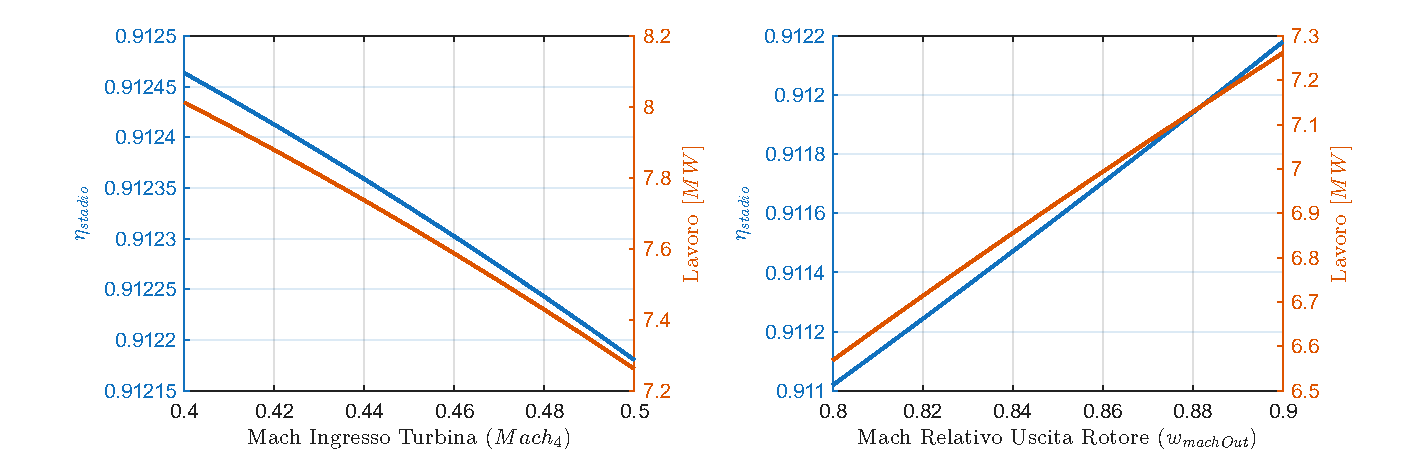
\includegraphics[width=1\linewidth]{Graphics/turbogetto/turbina/Analisi_Parametrica_Turbina__Effetto_Mach.pdf}
    \caption{(Sinistra) andamento del rendimento di stadio in funzione del numero di Mach all'ingresso della turbina.
    (Destra) andamento del rendimento di stadio in funzione del numero di Mach all'uscita del rotore.}
    \label{fig:turb:machRelativoEMachIngresso}
\end{figure}

\section{Ugello}
\label{appB:ugello}

Nel nostro caso viene considerato un ugello convergente-divergente con un rendimento \(\eta_{n}=0.95\) che opera in espansione ottima.
Nel caso il componente fosse ideale, la temperatura in uscita sarebbe:
\begin{equation*}
    T_{6_{\text{is}}} = T_{05} \text{NPR}^{\frac{1-\gamma}{\gamma}}
\end{equation*}
dove \(\text{NPR} = \frac{P_{05}}{P_{\text{amb}}}\).
Possiamo quindi ricavare il valore effettivo:
\begin{equation*}
    T_{6} = T_{05} - \eta_{n}(T_{05} - T_{06_{\text{is}}})
\end{equation*}
e trovare poi la velocità di efflusso con annesso numero di Mach:
\begin{equation*}
    u_{e} = \sqrt{2C_{p}(T_{05} - T_{6})}
\end{equation*}
\begin{equation*}
    M_{6} =\frac{u_{e}} {\sqrt{\gamma R T_{6}}}
\end{equation*}
Inoltre si ha la conservazione della temperatura totale e si ha, naturalmente, una variazione della pressione totale:
\begin{equation*}
    T_{06} =T_{05}
\end{equation*}
\begin{equation*}
    P_{06}=P_{05}(1 + \frac{\gamma-1}{2}M_{6}^2)^\frac{\gamma}{\gamma-1}
\end{equation*}
Per il dimensionamento delle aree di gola e di efflusso si fa affidamento alle seguenti formule:
\[ A^{\star}=\frac{\dot{m}\sqrt{RT_{06}}}{\Gamma P_{06}} \]
\[\frac{A_e}{A^{\star}}=\frac{1}{M_6} \left( \frac{1+\frac{\gamma-1}{2}M_6^{2}}{\frac{\gamma+1}{2}} \right)^{\frac{\gamma+1}{2(\gamma-1)}}\]


\section{Prestazioni}
\label{appB:prestazioni}
In regime subsonico le prestazioni del motore aerospaziale vengono calcolate a partire dalla velocità di volo $V_0$, dalla velocità di uscita dei gas dall'ugello $u_e$ e dalle rispettive portate di massa. I principali parametri di prestazione sono:

\textbf{Spinta} \\
\begin{equation*}
    F = \dot{m}_{\text{gas}} u_e - \dot{m}_{\text{aria}} V_0
\end{equation*}

\textbf{Consumo Specifico a Spinta (TSFC)} \\
Il consumo specifico di combustibile per unità di spinta $TSFC$ è espresso in $\left[\frac{\text{kg}}{\text{N} \cdot \text{h}}\right]$:
\begin{equation*}
    TSFC = \frac{\dot{m}_{\text{comb}}}{F} \cdot 3600
\end{equation*}

\textbf{Rendimenti del Motore} \\
I rendimenti descrivono la conversione dell'energia chimica del combustibile in potenza propulsiva:
\begin{itemize}
    \item \textbf{Rendimento Termico ($\eta_{\text{th}}$):} 
    \begin{equation*}
        \eta_{\text{th}} = \frac{\frac{1}{2} \dot{m}_{\text{gas}} u_{eq}^2 - \frac{1}{2} \dot{m}_{\text{aria}} V_0^2}{\dot{m}_{\text{comb}} LHV}
    \end{equation*}

    \item \textbf{Rendimento Propulsivo ($\eta_p$):} 
    \begin{equation*}
        \eta_p = \frac{F V_0}{\frac{1}{2} \dot{m}_{\text{gas}} u_{eq}^2 - \frac{1}{2} \dot{m}_{\text{aria}} V_0^2}
    \end{equation*}

    \item \textbf{Rendimento Globale ($\eta_g$):} 
    \begin{equation*}
        \eta_g = \eta_\text{th}\eta_p= \frac{F V_0}{\dot{m}_{\text{comb}} LHV}
    \end{equation*}
\end{itemize}

\textbf{Spinta Specifica}
\begin{equation*}
    F_s = \frac{F}{\dot{m}_{\text{aria}}}
\end{equation*}
La spinta specifica è il parametro di ottimizzazione utilizzato nel simulatore per ridurre le dimensioni del propulsore. 